\documentclass[a4paper]{article}

\usepackage{INTERSPEECH2021}

% Put the lab number of the corresponding exercise
\title{NLU course project}
\name{Gianluigi Vazzoler (257846)}
\address{University of Trento}
\email{gianluigi.vazzoler@studenti.unitn.it}

\usepackage{graphicx}
\graphicspath{{plots/}}

\begin{document}

\maketitle

\section{Introduction}
This report describes the second part of the NLU course project, which focuses on intent classification and slot filling using the ATIS dataset. In Part 2.A, the baseline LSTM architecture is enhanced with bidirectional layers and dropout regularization to improve both intent classification accuracy and CoNLL-style slot F1 score. In Part 2.B, a pre-trained BERT model is fine-tuned within a multi-task learning framework for joint intent and slot prediction \cite{devlin2019bert, chen2019bert}. Each configuration is repeated over three runs to report mean and standard deviation.
\section{Implementation details}

\subsection{Part 2.A: LSTM with Bidirectional Layers and Dropout}

\begin{itemize}
  \item \textbf{Bidirectionality:} 
    The encoder was configured to process each utterance in two directions—forward and backward—so that the hidden representations capture contextual dependencies both from past and future tokens. As a result, the downstream slot‐tagging and intent‐classification layers receive twice the usual hidden size, ensuring they leverage information from both directions.

  \item \textbf{Dropout:}
    To improve generalization, dropout was applied at two points in the network. First, a dropout layer follows the embedding layer, randomly zeroing some token embeddings during training. Second, another dropout layer is applied to the LSTM’s output representations before they feed into the slot and intent classifiers. A dropout probability in the range of \{0.1, 0.5\} was used.
\end{itemize}

\subsection{Part 2.B: BERT-based Multi-task Learning (Sub-Token Challenge)}

Unlike the LSTM approach, BERT relies on WordPiece (byte-pair) tokenization, which can split single words into multiple sub-tokens. To address this alignment challenge, all experiments (both BERT-base and BERT-large) are conducted using the same pipeline, and results are reported as mean \(\pm\) standard deviation over three seeds (42, 43, 44).

\begin{itemize}
  \item \textbf{Byte-Pair Encoding (WordPiece):} Each input sentence is tokenized into sub-tokens (e.g., “San Francisco” might become \texttt{\{``San'', ``Franc'', ``\#\#isco''\}}). Because slot tags are defined at the word level, naively assigning a tag to every sub-token would misalign labels.
  \item \textbf{First Sub-Token Labeling:} Using the tokenizer’s \texttt{word\_ids()} mapping, the implementation identifies which sub-tokens belong to the same original word. Only the first sub-token of each word is assigned the true slot label; all subsequent sub-tokens receive a special \texttt{PAD\_TOKEN} label (ignored during loss computation).
  \item \textbf{Resulting Alignment:} This strategy ensures that slot labels remain consistent even when words are broken into multiple sub-tokens. The BERT encoder processes all sub-tokens, but during training and evaluation, only the logits corresponding to each word’s first sub-token contribute to the slot-filling loss.  
  \item \textbf{Intent Classification head:} The pretrained BERT encoder (either \texttt{bert-base-uncased} or \texttt{bert-large-uncased}) is used to obtain contextual representations over all sub-tokens \cite{devlin2019bert, huggingface-bert}. The hidden state corresponding to \texttt{[CLS]} is passed through a dropout layer (with \(p=0.1\)) and a linear layer, producing logits for each intent \cite{chen2019bert}. A softmax yields the final intent prediction.
\end{itemize}



\section{Results}
Performance was assessed using intent accuracy and slot-filling F1 score (mean \(\pm\) std over three runs with seeds 42, 43, 44).

\begin{itemize}
  \item \textbf{Part 2.A (LSTM):} 
    Table~1 reports results for unidirectional and bidirectional LSTM variants, each with three runs. Adding bidirectionality alone raises Slot F1 from 0.914~\(\pm\)~0.030 to 0.936~\(\pm\)~0.003 (Intent Acc 0.934~\(\pm\)~0.080 $\rightarrow$ 0.940~\(\pm\)~0.002). Introducing dropout \(p=0.1\) further improves to 0.940~\(\pm\)~0.003 (Intent Acc 0.948~\(\pm\)~0.002). Higher dropout (\(p=0.3\), \(p=0.5\)) yields marginal variations, confirming that light regularization (0.1--0.3) is optimal on ATIS.
  \item \textbf{Part 2.B (BERT):} 
    Table~2 compares BERT-base and BERT-large (each averaged over three runs). BERT-base achieves Slot F1 0.954~\(\pm\)~0.001, Intent Acc 0.974~\(\pm\)~0.0005. Switching to BERT-large raises Slot F1 slightly to 0.958~\(\pm\)~0.001 and Intent Acc to 0.976~\(\pm\)~0.001, indicating a small but consistent improvement from increased model capacity.
\end{itemize}

Together, these results (Table~1 and Table~2) show that (1) capturing bidirectional context and (2) applying modest dropout significantly boost LSTM performance, while (3) leveraging pretrained transformers (especially BERT-large) yields the highest Slot F1 and Intent Accuracy on ATIS.

\bibliographystyle{IEEEtran}
\bibliography{mybib}

\clearpage
\onecolumn

\begin{table}[ht]
  \centering
  \begin{tabular}{lcc}
    \hline
    \textbf{Architecture}                          & \textbf{Slot F1}       & \textbf{Intent Acc}    \\
    \hline
    ModelIAS (unidirectional, no dropout)         & 0.914 ± 0.03                & 0.934 ± 0.08                 \\
    ModelIAS (bidirectional, no dropout)          & \textbf{0.936} ± \textbf{0.003}                 & \textbf{0.940} ± \textbf{0.002}                 \\
    \midrule
    ModelIAS (bidir + drop (p=0.1))            & \textbf{0.940} ± \textbf{0.003} & \textbf{0.948} ± \textbf{0.002} \\
    ModelIAS (bidir + drop (p=0.3))            & 0.939 ± 0.004 & 0.946 ± 0.002 \\
    ModelIAS (bidir + drop (p=0.5))            & 0.932 ± 0.0004 & 0.948 ± 0.004 \\
    \hline
  \end{tabular}
  \vspace{2em}
  \caption{Part 2.A Results. “ModelIAS” = unidirectional LSTM without dropout; “bidirectional” = two‐way LSTM without dropout; “bidirectional + dropout” = two‐way LSTM with dropout (mean ± std over three runs).}
\end{table}

\vspace{-10pt}

\begin{table}[ht]
  \centering
  \begin{tabular}{lcc}
    \hline
    \textbf{Architecture}                             & \textbf{Slot F1} & \textbf{Intent Acc} \\
    \hline
    JointModel (BERT‐base‐uncased)                    & 0.954 ± 0.001   & 0.974 ± 0.0005      \\
    JointModel (BERT‐large‐uncased)                    & \textbf{0.958 ± 0.001}   & \textbf{0.976 ± 0.001}      \\
    \hline
  \end{tabular}
  \vspace{2em}
  \caption{Part 2.B Results, each averaged over 3 runs. Both base and large BERT models were used.}
\end{table}

\begin{figure}[htbp!]
  \centering
  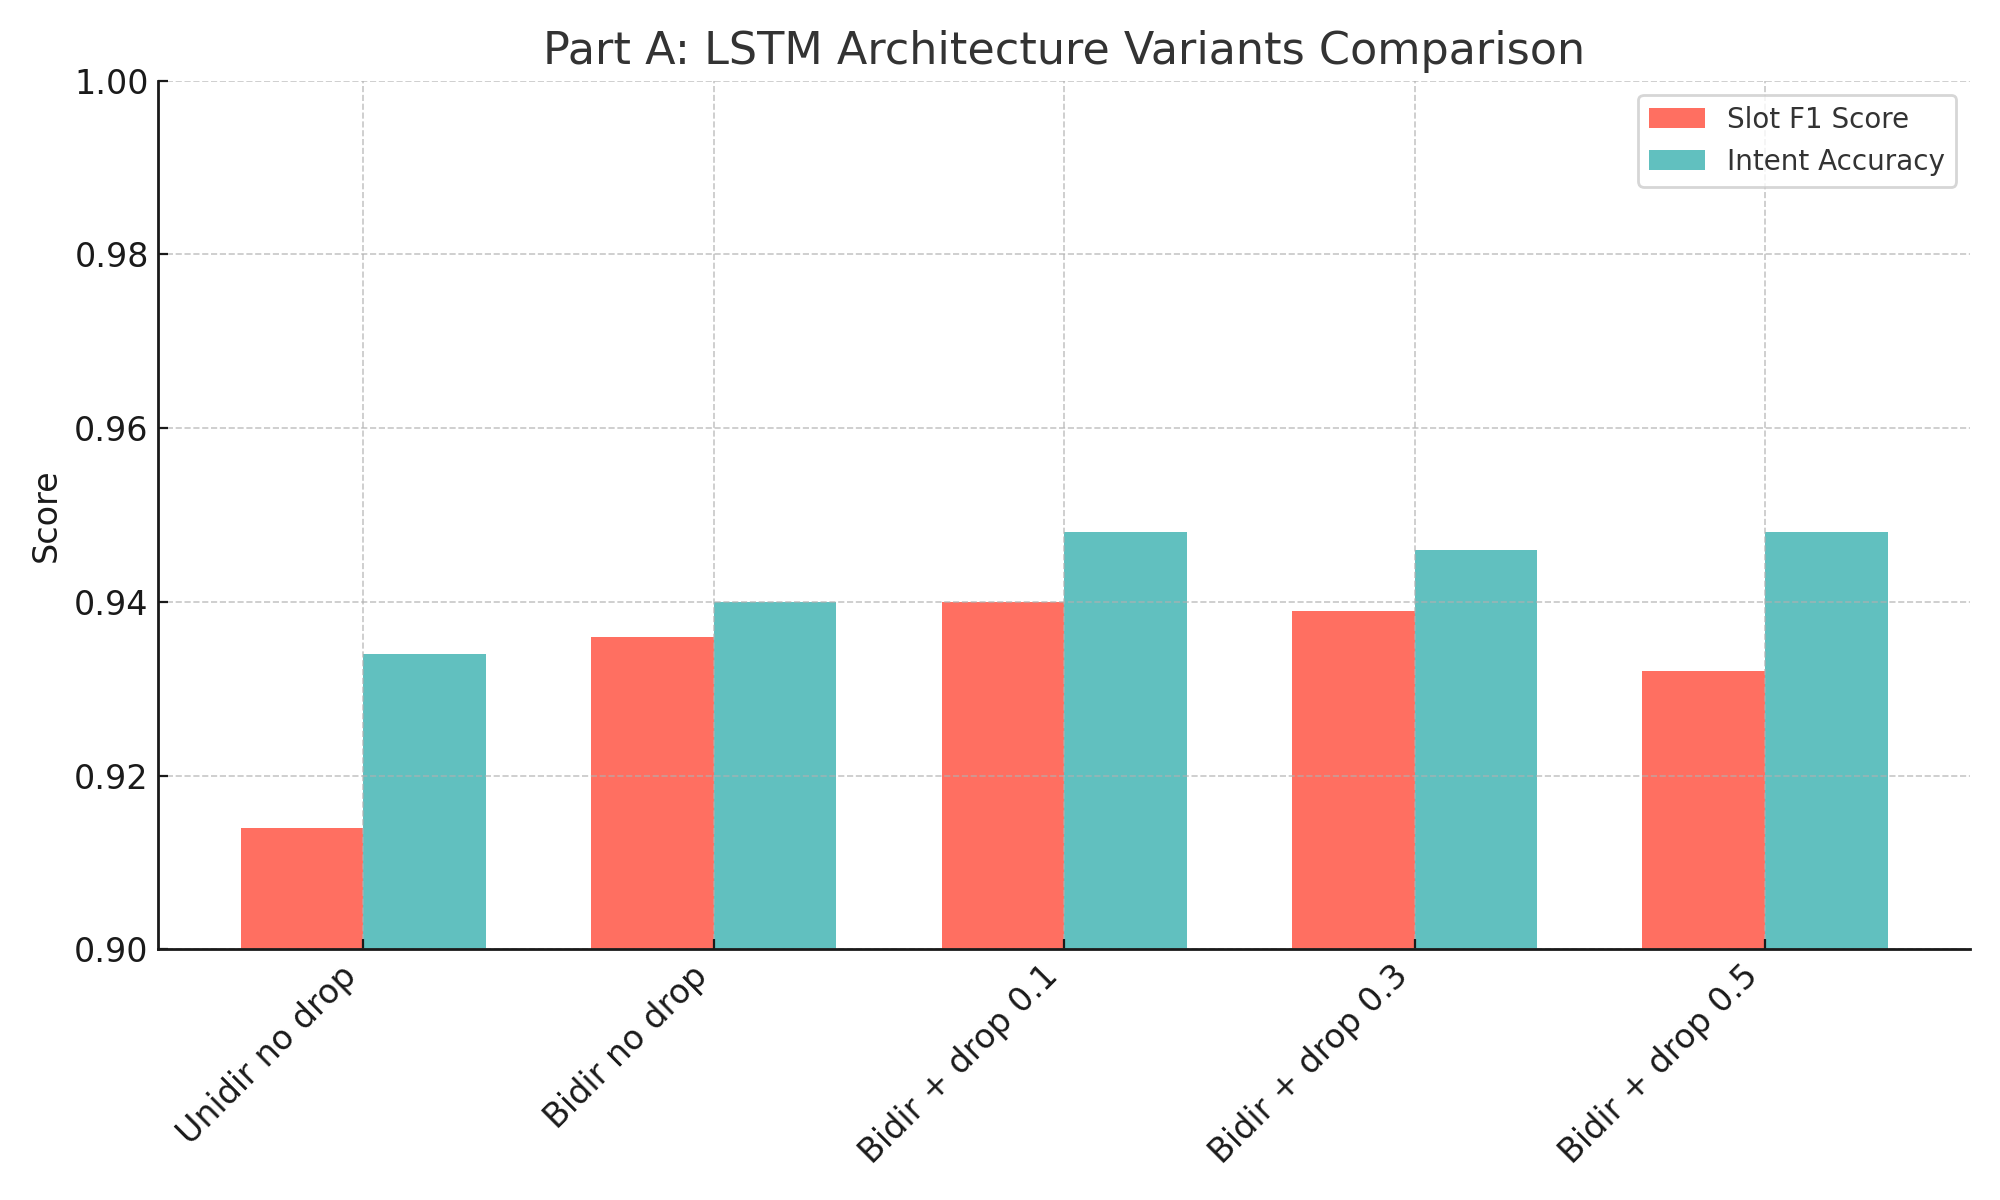
\includegraphics[width=0.6\linewidth]{partA_comparison.png}
  \caption{Performance comparison of LSTM models (Part 2.A) with different configurations on slot F1 and intent accuracy.}
  \label{fig:lstm_performance}
  \vspace{-10pt}
\end{figure}

\vspace{2em}

\begin{figure}[htbp!]
  \centering
  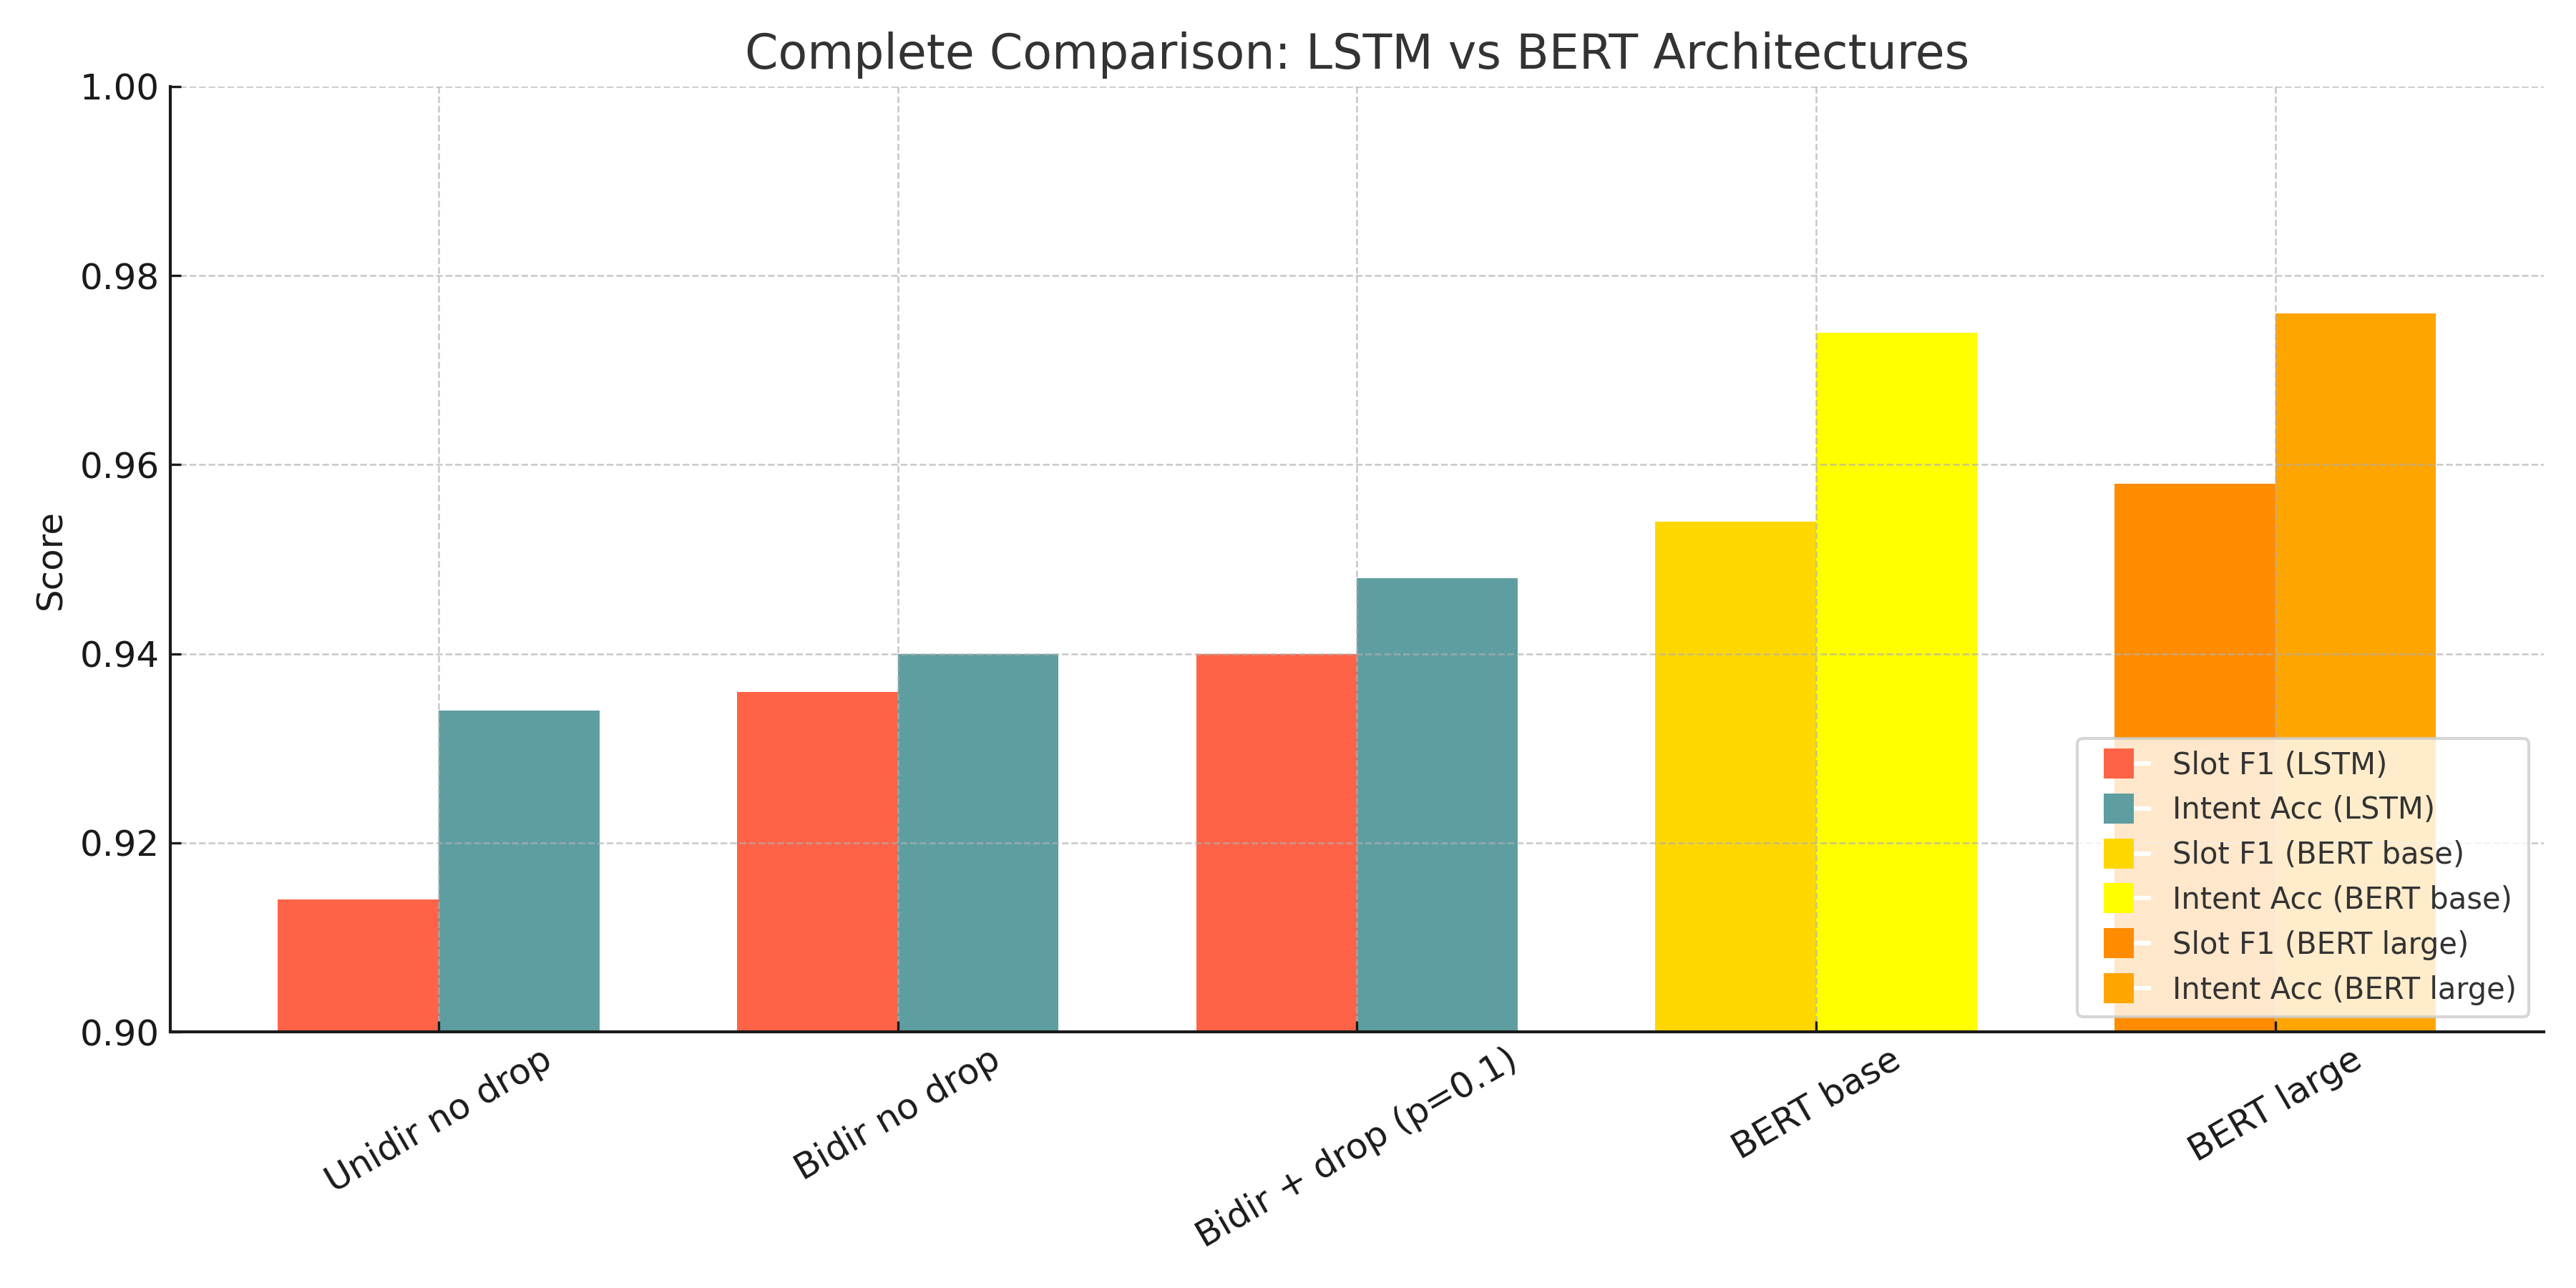
\includegraphics[width=0.7\linewidth]{complete_comparison.png}
  \caption{Performance of the BERT-based joint models (Part 2.B) with respect to the other LSTM configurations (Part 2.A).}
  \label{fig:bert_performance}
\end{figure}


\end{document}
